\documentclass[article,colorback,accentcolor=tud4c]{tudreport}
\usepackage{ngerman}

\usepackage[stable]{footmisc} 
\usepackage[ngerman]{hyperref}
\usepackage[utf8]{inputenc}
\usepackage{longtable}
\usepackage{multirow}
\usepackage{booktabs}
\usepackage{pst-all}
\usepackage{amsmath}
\usepackage{subfigure}


% Makros
\newcommand{\before}[1]{\textit{ before(#1) }}
\newcommand{\after}[1]{\textit{after(#1)}}
\newcommand{\aktiv}[1]{\textit{active(#1)}}
\newcommand{\Interval}[1]{\textbf{interval#1}}
\newcommand{\comp}[1]{\textit{comp(#1)}}
\newcommand{\val}[1]{\textit{value(#1)}}

\hypersetup{%
  pdftitle={TUD Corporate-Design f"ur {\LaTeX}}, pdfauthor={C. v. Loewenich und
  J. Werner}, pdfsubject={Beispieltext}, pdfview=FitH, pdfstartview=FitV }

\setcounter{seclinedepth}{1}

  \newif\ifTUDmargin\TUDmarginfalse \ifTUDmargin\makeatletter
    \TUD@setmarginpar{2}
  \makeatother\fi

\newlength{\longtablewidth}
\setlength{\longtablewidth}{0.7\linewidth}
\addtolength{\longtablewidth}{-\marginparsep}
\addtolength{\longtablewidth}{-\marginparwidth}

\title{IntervalEvents in EScala: Design}
\subtitle{Michael Kutschke und Frank Englert}

\begin{document}

\maketitle

\tableofcontents

\section{Grundlegende Definitionen}
\label{definitions}
Sei \before{\Interval} : Event das Ereignis, das den Beginn des Intervalls int angibt
und \after{\Interval} : Event jenes, welches das Ende des Intervalls angibt.
Hierbei sind folgende Event-Sequenzen zulässig:
\begin{itemize}
\item einmal \before{\_} zu Beginn und einmal \after{\_} am Ende
\item mehrfaches \before{\_} und ein \after{\_} am Ende 
\item verschachtelte, paarweise passende \before{\_} und \after{\_} Ereignisse
%\item beliebige \before{\_} und \after{\_} Events innerhalb des Intervals
\end{itemize}
Ausserdem gebe \aktiv\Interval{} : boolean an, ob das Intervall aktiv ist.
In der jetzigen Fassung bedeutet dies einfach, ob man sich zeitlich innerhalb des
Intervalls befindet. 
Der Wert des Active-Flags hat dabei die in Abb.
\ref{active_bit_behaviour} gezeigte Semantik. Zum Zeitpunkt des
Before-Events ist \aktiv\Interval{} noch nicht gesetzt. Dies ist keine
Einschr"ankung, wie im weiteren gezeigt werden wird. 

\begin{figure}[h]
 \centering 
\psset{unit=1cm} 
\begin{pspicture}(0,0)(10,2)
\psgrid[subgriddiv=1,griddots=10,gridlabels=7pt,](0,0)(10,2)
%{
%	\pspolygon[fillcolor=greenyellow,fillstyle=solid,linestyle=none](0,0)(0,1)(1,1)(1,0)

	\rput(1.2,0.7){\psframebox*[framearc=.3]{B}}
	\rput(9.2,0.7){\psframebox*[framearc=.3]{A}}
	\rput(0.2,1.05){\psframebox*[framearc=.3]{Aktiv}} 
	\psline[linewidth=1pt]{]-]}(1,1)(9,1)
%}
\end{pspicture}
\caption{Wert des Aktiv-Bits}
\label{active_bit_behaviour}
\end{figure}


F"ur alle Intervalle muss gelten, dass active nur beim \before{\_} oder
\after{\_} Event umgeschaltet wird, wobei \aktiv{\_} nur von einem \before{\_}
Event gesetzt und von einem \after{\_} Event zur"uckgesetzt werden kann.
Ausserdem sollten ausserhalb des Intervalls keine isolierten Events auftreten.

\section{Operatoren}
Im folgenden werden die auf Intervall-Events verfügbaren Operatoren definiert:

\subsection{Komplement \comp\Interval : Intervall}
\begin{itemize}
\item \before{\comp{\Interval}} <=> \after{\Interval}
\item \after{\comp{\Interval}} <=> \before{\Interval} 
\item \aktiv{\comp{\Interval}} <=> ! \aktiv{\Interval}
\end{itemize}
Bei der Implementierung wird ein neues Intervall-Event erzeugt, bei dem das 
Before-Event mit dem After-Event getauscht ist. Das Komplement bietet keinen
Zugriff auf den Value des Intervall-Events.

\subsection{Vereinigung \Interval{1} || \Interval{2} : Intervall}
Die Semantik der ||-Vereinigung ist die Vereinigung der Zeitpunkte von
\Interval{1} und \Interval{2}.
\begin{itemize}
\item \before{\Interval{1} || \Interval{2}}  <=> (\before{\Interval{1}} ||
\before{\Interval{2}}) \&\& !
\aktiv{\Interval{1} || \Interval{2}}
%(((after && (_ => !ie.active)) || 
% (ie.after && (_ => !active)) || 
% (after and ie.after))) \ (before || ie.before), active || 
% ie.active, _value)
\item \after{\Interval{1} || \Interval{2}} <=> \after{\Interval{1}} \&\&
!\aktiv{\Interval{2}} || \after{\Interval{2}} \&\& !\aktiv{\Interval{1}} ||
\after{\Interval{1}} \&\& \after{\Interval{2}}except(\before{\Interval{1}}||\before{\Interval{2}})

\end{itemize}

\subsection{Schnitt \Interval{1} \&\& \Interval{2} : Intervall}
\begin{itemize}
\item \before{\Interval{1} \&\& \Interval{2}} <=> (((\before{\Interval{1}} \&\& \aktiv{\Interval{2}}) ||
(\before{\Interval{2}} \&\& \aktiv{\Interval{1}}) || (\before{\Interval{1}} \&\& \before{\Interval{2}}))
\textbackslash (\after{\Interval{1}} || \after{\Interval{2}})) \&\& ! \aktiv{\Interval{1} \&\& \Interval{2}}
\item \after{\Interval{1} \&\& \Interval{2}} <=> \before{\comp{\Interval{1}}} ||
\before{\comp{\Interval{2}}}
\item \aktiv{\Interval{1} \&\& \Interval{2}} <=> \aktiv{\Interval{1}} \&\& \aktiv{\Interval{2}}
\end{itemize}

\subsection{Differenz \Interval{1} \textbackslash\ \Interval{2} : Interval}
Alle Zeitpunkte, die in \Interval{1} liegen, nicht aber in \Interval{2}:
\begin{itemize}
  \item  \Interval{1} \textbackslash\ \Interval{2} <=> \Interval{1} \&\&
  comp(\Interval{2})
\end{itemize}


\subsection{within(\Interval{},e) : Event}
within(\Interval{},e) <=> (e \&\& \aktiv{\Interval}) || (e \&\& \before{\Interval})

\subsection{!within(\Interval{},e) : Event}
!within(\Interval{},e) <=> (e \&\& ! \aktiv{\Interval}) \textbackslash\ \before{\Interval}

\subsection{ StrictlyWithin(\Interval{},e) : Event}
StrictlyWithin(\Interval{},e) <=> (e \&\& \aktiv{\Interval}) \textbackslash\ \after{\Interval}

\subsection{ !strictlyWithin(\Interval{},e) : Event }
!strictlyWithin(\Interval{},e) <=> (e \&\& ! \aktiv{\Interval}) || (e \&\& \after{\Interval})


\subsection{weitere Anmerkungen}
Der Umstand, dass sich int und \comp{\Interval{}} zwei Zeitpunkte teilen, mag
unintuitiv erscheinen, allerdings  bietet dies nicht nur Nachteile. So ist int
|| \comp{\Interval{}} wie  erwartet immer aktiv, beginnt und endet niemals. int
\&\& \comp{\Interval{}} ist niemals aktiv  und l"ost auch niemals before oder
after Ereignisse aus.

  \section{An Events gebundene Werte}
Es ist m"oglich, beliebige Werte an Events zu binden. Diese M"oglichkeit
existiert auch f"ur Intervall-Events. Wann im Intervall welche Werte
gelten, h"angt von der Art des Intervalls ab. 

Auf den aktellen Wert des Intervalls wird "uber \val(\Interval{})
zugegriffen. 

Nachfolgend wird das Standartverhalten der Intervall-Operatoren dargestellt.
Allerdings kann das Verhalten der Operatoren bei Bedarf abge"andert werden. Dann
muss beim Intervall-Event-Knoten eine Benutzerdefinierte Merge-Funktion
angegeben werden, die Values der Events aggregiert.

\subsection{Intervall zwischen dem Event B und dem Event A)}
F"ur between-Intervalle wie in Abbildung \ref{interval-between_b_a} gilt der Wert des
Before-Events bis zum End-Event. Dannach hat das Intervall den Wert null. Der
Wert des After-Events wird allerdings nicht im Komplement gespeichert. Beim
Intervall\ref{interval-between_b_a} gilt also:
\[
val(t) = \begin{cases}
null & t < 1 \\
B.val & t >= 1 \; and \; t < 9 \\
null & t >= 9
\end{cases}
\]

\begin{figure}[h]
 \centering 
\psset{unit=1cm}
\begin{pspicture}(0,0)(10,2)
\psgrid[subgriddiv=1,griddots=10,gridlabels=7pt](0,0)(10,1)
%{
%	\pspolygon[fillcolor=greenyellow,fillstyle=solid,linestyle=none](0,0)(0,1)(1,1)(1,0)

	\rput(1.2,0.7){\psframebox*[framearc=.3]{B}}
	\rput(9.2,0.7){\psframebox*[framearc=.3]{A}}
	\psline[linewidth=1pt]{[-]}(1,0.5)(9,0.5)
%}
\end{pspicture}
\caption{Intervall-Event between(B,A)}
\label{interval-between_b_a}
\end{figure}



Wenn die \before{\_}-Events mehrfach auftreten, hat das
between-Intervall den Wert des ersten \before{\_}-Events. Ein Beispiel hierf"ur ist in Abbildung
\ref{interval-between_b_a-multiple} zu sehen. F"ur
Interval\ref{interval-between_b_a-multiple} gilt \[ val(t) =
\begin{cases}
null & t < 1\\
B.val &  t >= 1 \; and \; t < 7\\
null  & t >= 7
\end{cases}
\]

\begin{figure}[h]
 \centering 
\psset{unit=1cm}
\begin{pspicture}(0,0)(10,2)
\psgrid[subgriddiv=1,griddots=10,gridlabels=7pt](0,0)(10,1)
%{
	\rput(1.2,0.75){\psframebox*[framearc=.3]{B}}
	\rput(7.2,0.75){\psframebox*[framearc=.3]{A}}
	\psline[linewidth=1pt]{[-]}(1,0.5)(7,0.5)
	
	\rput(3.2,0.75){\psframebox*[framearc=.3]{B'}}
	\rput(9.2,0.75){\psframebox*[framearc=.3]{A'}}
	\psline[linewidth=1pt,linestyle=dotted]{[-]}(3,0.5)(9,0.5)
%}
\end{pspicture}
\caption{Intervall-Event between(B,A) mit mehrfach auftretenden Before- und
After-Events}
\label{interval-between_b_a-multiple}
\end{figure}
 
 
\subsection{Vereinigung von Intervallen}
F"ur die Vereinigung von Intervallen ist es sinnvoll, den Wert des letzen
\before{\_}-Events zu speichern. Damit hat man immer Zugriff auf den Wert des
letzten Events, der die Bedingung erf"ullt hat. 

\begin{figure}[h]
 \centering 
\psset{unit=1cm}
\begin{pspicture}(0,0)(10,4)
\psgrid[subgriddiv=1,griddots=10,gridlabels=7pt](0,0)(10,3)
%{
	\rput(1.2,2.75){\psframebox*[framearc=.3]{B}}
	\rput(7.2,2.75){\psframebox*[framearc=.3]{A}}
	\psline[linewidth=1pt]{[-]}(1,2.5)(7,2.5)
	
	\rput(3.2,1.75){\psframebox*[framearc=.3]{B'}}
	\rput(9.2,1.75){\psframebox*[framearc=.3]{A'}}
	\psline[linewidth=1pt]{[-]}(3,1.5)(9,1.5)
	
	\rput(1.2,0.75){\psframebox*[framearc=.3]{B}}
	\rput(9.2,0.75){\psframebox*[framearc=.3]{A'}}
	\psline[linewidth=1pt]{[-]}(1,0.5)(9,0.5)
%}
\end{pspicture}
\caption{Vereinigung zweier Intervall-Events: between(B,A) || between(B',A')}
\label{interval-or}
\end{figure}
  
F"ur das in Abb\ref{interval-or} zu sehende Interval\ref{interval-or}
between(A,B) || between(A',B') gilt also die folgende Belegung des Wertes:
\[
val(t) = \begin{cases}
null & t < 1 \\
B.val & t >=1 \; and t < 3 \\
B'.val & t >=3 \; and t < 9 \\
null & t > 9 \\
\end{cases}
\]
  
  \subsection{Schnittmenge zwischen Intervallen}
Bei der Schnittmenge zwischen zwei Intervall-Events werden die Event-Werte der
beiden aktiven Interval-Events zu einem Tupel zusammengefasst. 

\begin{figure}[h]
 \centering 
\psset{unit=1cm}
\begin{pspicture}(0,0)(10,4)
\psgrid[subgriddiv=1,griddots=10,gridlabels=7pt](0,0)(10,3)
%{
	\rput(1.2,2.75){\psframebox*[framearc=.3]{B}}
	\rput(7.2,2.75){\psframebox*[framearc=.3]{A}}
	\psline[linewidth=1pt]{[-]}(1,2.5)(7,2.5)
	
	\rput(3.2,1.75){\psframebox*[framearc=.3]{B'}}
	\rput(9.2,1.75){\psframebox*[framearc=.3]{A'}}
	\psline[linewidth=1pt]{[-]}(3,1.5)(9,1.5)
	
	\rput(3.2,0.75){\psframebox*[framearc=.3]{(B,B')}}
	\rput(7.2,0.75){\psframebox*[framearc=.3]{(A', A)}}
	\psline[linewidth=1pt]{[-]}(3,0.5)(7,0.5)
%}
\end{pspicture}
\caption{Schnittmenge zweier Intervall-Events: between(B,A) and
between(B',A')}
\label{interval-and}
\end{figure}

Wie in Abb. \ref{interval-and} zu sehen, ergibt sich das folgende Zeitliche
Verhalten f"ur den Wert von Interval\ref{interval-and} \[
val(t)=\begin{cases}
null & t < 3 \\
(B,B') & t >=3 \; and t <= 7 \\
null & t > 7
\end{cases}
\]

\subsection{Differenz zweier Intervall-Events}
Bei der Differenz zwischen zwei Intervall-Events ist der Wert des Intervalls
gleich dem Wert des letzten Before-Events vor oder nach dem Schnitt.

\begin{figure}[h]
 \centering 
\psset{unit=1cm}
\begin{pspicture}(0,0)(10,4)
\psgrid[subgriddiv=1,griddots=10,gridlabels=7pt](0,0)(10,3)
%{
	\rput(1.2,2.75){\psframebox*[framearc=.3]{B}}
	\rput(4.2,2.75){\psframebox*[framearc=.3]{A}}
	\psline[linewidth=1pt]{[-]}(1,2.5)(4,2.5)
	
	\rput(6.2,2.75){\psframebox*[framearc=.3]{B''}}
	\rput(9.2,2.75){\psframebox*[framearc=.3]{A''}}
	\psline[linewidth=1pt]{[-]}(6,2.5)(9,2.5)
	
	\rput(3.2,1.75){\psframebox*[framearc=.3]{B'}}
	\rput(5.2,1.75){\psframebox*[framearc=.3]{A'}}
	\psline[linewidth=1pt]{[-]}(3,1.5)(5,1.5)
	
	\rput(1.2,0.75){\psframebox*[framearc=.3]{B}}
	\rput(3.2,0.75){\psframebox*[framearc=.3]{B'}}
	\psline[linewidth=1pt]{[-]}(1,0.5)(3,0.5)
	
	\rput(6.2,0.75){\psframebox*[framearc=.3]{B''}}
	\rput(9.2,0.75){\psframebox*[framearc=.3]{A''}}
	\psline[linewidth=1pt]{[-]}(6,0.5)(9,0.5)
%}
\end{pspicture}
\caption{between(B,A) except between(B',A')}
\label{interval-diff}
\end{figure}

F"ur Interval\ref{interval-diff} = between(B,A) except between(B', A') ergibt
sich also folgende Belegung:
\[
val(t)=\begin{cases}
null & t < 1 \\
B & t \in [1,3] \\
null & t \in [3,6] \\
B'' & t\in[6,9]\\
null & t >9
\end{cases}
\]

\section{Implementierung}

Die Implementierung der Interval-Events hat das gleiche Schema wie die
Implementierung der Events. Es handelt sich bei Intevall-Events um eine
spezielle Form von Event-Nodes die aus einem Start- und einem Stop-Event
bestehen.

Wie bei jedem Event-Node aus dem scala.events-Package durchläuft ein
Intervall-Event einen Lebenszyklus bestehend aus dem Setup des Event-Graphen,
der Registrierung von Reactions, dem Deploy, der Unregistrierung von Reactions
und dem Undeploy von Event-Nodes. Dieser Lebenszyklus ist auch in
Abb. \ref{event_node_lifecycle} zu sehen.

%\usepackage{graphics} is needed for \includegraphics
\begin{figure}[htp]
\begin{center}
  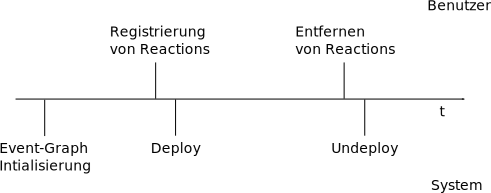
\includegraphics[width=0.7\textwidth]{graphics/EventNode-Lifecycle}
  \caption{Lifecycle eines EventNodes}
  \label{event_node_lifecycle}
\end{center}
\end{figure}


Es gibt, wie in Abb. \ref{interval_events_structure} zwei Klassen von
Interval-Event-Nodes: BetweenEvents und ExecutionEvents. BetweenEvents sind vom
Auftreten des StartEvents bis zum Auftreten des ersten End-Events aktiv, wenn
eine Reaction registiert wurde. Das Execution-Event dient dazu, die Ausführung
einer Funktion zu protokollieren. Wenn das Execution-Event eine Funktion
überwachen soll, dann instrumentiert der Compiler die Funktion so, dass ein
Before-Event beim Betreten der Funktion und ein After-Event beim Verlassen der
Funktion ausgelöst wird.

%\usepackage{graphics} is needed for \includegraphics
\begin{figure}[htp]
\begin{center}
  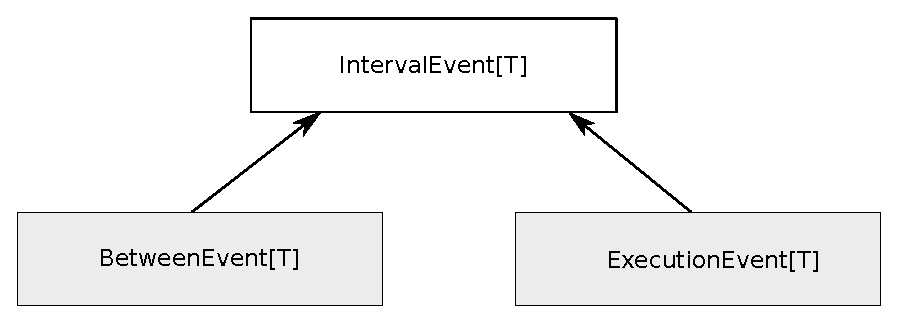
\includegraphics[width=0.5\textwidth]{graphics/interval_event_structure}
  \caption{Arten von Intervall-Events}
  \label{interval_events_structure}
\end{center}
\end{figure}


\subsection{Der Aufbau des Event-Graphen}
Mithilfe von Event-Nodes können mehrere Events zu komplexeren Events
zusammengefasst werden. So ist es beispielsweise möglich, alle Events einer
Filter-Bedingung zu unterziehen. Das resultierende Event wird nur dann
ausgelöst, wenn ein zu filterndes Event auftritt dessen Filterbedingung zu true
auswertet. 

Der daraus resultierende Abhänigkeitsgraph soll nachfolgend als Event-Graph
bezeichnet werden.

Intervall-Events können uneingeschränkt auch als Knoten im Event-Graph
vorkommen. Eine Liste der möglichen Filterfunktionen und die dazugehörigen
Definitionen findet sich im Kapitel \ref{definitions}.

\subsection{Auswertung des Event-Graphen}

Bei der Auswertung eines Event-Graphen gibt es zwei möglichen Vorgehensweisen.
Zum einen kann Events sammeln, die bei Event-Graphen ankommen und dann
weiterleiten, wenn gewisse Bedingungen erfüllt sind. Hierbei handelt es sich um
eine Push-basierte Implementierungen. Es werden nämlich nur Änderungen gepusht.

Beim Zweiten Ansatz werden keien Ändeurngen weitergeleitet. Stattdessen wird der
Event-Graph traversiert um herauszufinden, ob Änderungen passiert sind. Dieser
Ansatz wird nachfolgend als pull-Basiert bezeichnet.

Bei gleichem Resultat haben beide Implementierungen verschiedene Vor- und
Nachteile. Nateilig beim Push-Basierten Ansatz ist die relativ hohe Komplexität
der Implementierung wenn Knoten im Event-Graph einen Zustand aufweisen.
Außerdem ist es schwierig, ein deterministisches Verhalten sicherzustellen. Beim
Pull-basierten Ansatz stellt sich stattdessen die Frage, wie man den richtigen
Zeitpunkt für einen Pull ermitteln kann. 

Die Implementierung im scala.events-Modul verwendet einen hybriden Ansatz um den
Event-Graphen auszuwerten. Die meisten Event-Knoten wurden Push-Basiert
implementiert. Eine Ausnahme stellt der Except-Knoten dar. Mit einem
Event-Knoten können verschiedene Events ausgeschlossen werden. Der Except-Zweig
des Event-Knotens wurde pull-basiert implementiert.

Betrachten wir nachfolgend zwei Beispiele um diese Vorgehensweise zu begründen:
\begin{eqnarray}
val \; e & = e1 \setminus (e2 || e3)\\
val \; e & = e1 \setminus (e1 || e3)
\end{eqnarray}

Der Event-Graph des Push-basierten Ansatzes ist in
Abb\ref{push_based_event_graph} zu sehen.

%\usepackage{graphics} is needed for \includegraphics
\begin{figure}[htp]
\centering
\subfigure[Push basierter Event-Gaph] {
  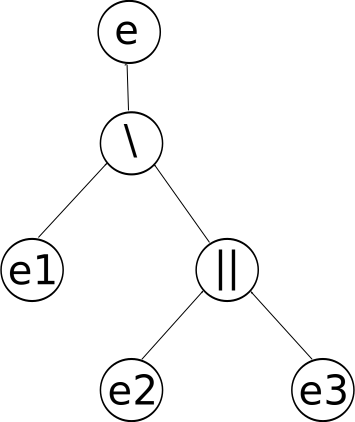
\includegraphics[width=0.3\textwidth]{graphics/event_node_except_push}
  \label{push_based_event_graph}
}
\subfigure[Push/Pull basierter Event-Graph] {
  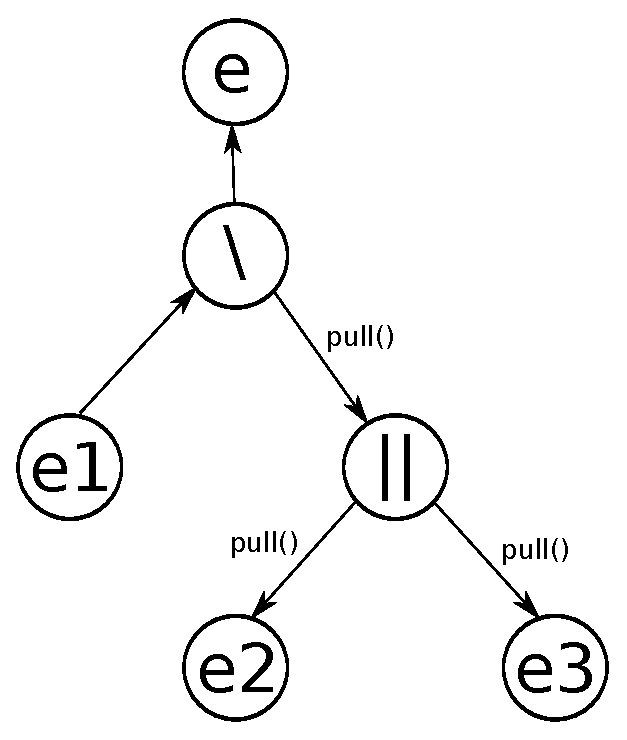
\includegraphics[width=0.3\textwidth]{graphics/event_node_except_pull}
  \label{pull_based_event_graph}
}
\caption{Event-Graphen für das Beispiel 1}
\end{figure}

\begin{figure}[htp]
\centering
\subfigure[Push basierter Event-Gaph] {
  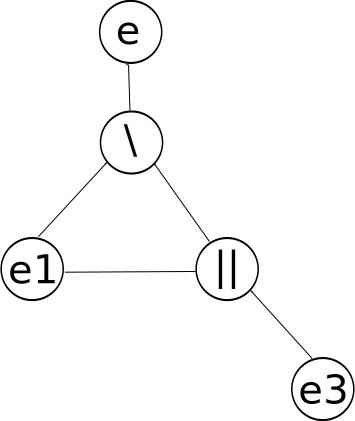
\includegraphics[width=0.3\textwidth]{graphics/event_node_except2_push}
  \label{failing_push_based_event_graph}
}
\subfigure[Push/Pull basierter Event-Graph] {
  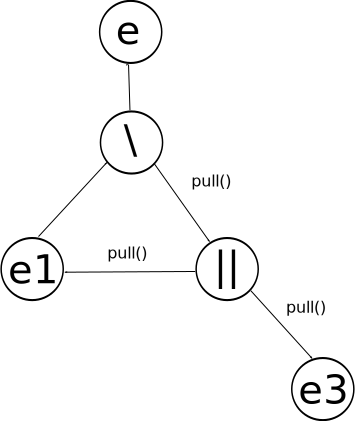
\includegraphics[width=0.3\textwidth]{graphics/event_node_except2_pull}
  \label{working_pull_based_event_graph}
}
\caption{Event-Graphen für das Beispiel 2}
\end{figure}


\subsubsection{Einschränkungen der Implementierung}
In einem Event-Graph können nicht EventNodeRef oder EventNodeExists in einem
Pfad zusammen mit EventNodeExcept verwendet werden, da dies möglicherweise zu
nicht korrekten Ergebnissen führen würde.

Beim EventNodeExcept kann ein Except-Event empfangen werden, der das Entfernen
von Reactions auslöst. Die sorgt möglicherweise für Inkonsistenzen
bei Vorgängerknoten im Event-Graphen, wenn sich die Reaction des Except-Knotens
vor der Reaction eines anderen Knotens in der ReactionListe befindet.
Daher muss im Falle eines Except-Events immer ein Undeploy und ein Deploy
ausgeführt  werden, um die geänderten Reactions weiterzupropagieren.

Dies funktioniert allerdings nicht mehr länger mit EventNodeRef oder
EventNodeExists, dieses die Reihenfolge von Reactions verändern können.

\section{Beispiele}
\subsection{Implementierung eines Zustandsautomaten}
Zwei Beispiele zeigen die Verwendung von Intervall-Events bei der
Implementierung von Zustandsautomaten. Zustandsautomaten k"onnen hervoragend
durch die Verwendung von IntervallEvents implementiert werden, da
Zustandsautomaten immer vom Zustand abh"anige Reaktionen auf Events zeigen.

Zur Implementierung kann jeder Zustand des Automaten als ein Intervall
abgebildet werden. Nun kann man Entry-Actions als before-Event an ein Intervall
und Exit-Actions als ein after-Event an das Intervall binden. Transition-Actions
k"onnen wahlweise an das Before- oder das After-Event gebunden werden.
Self-Transitions werden als Vereinigung zwischen dem Intervall-Event und dem
ausl"osenden Event der Self-Transition abgebildet. 

Durch diese Vorgehensweise ergibt sich eine bessere Wartbarkeit des
Quellcodes, da das Programmverhalten nicht mehr imperativ durch If-Statements
oder das Statemachine-Pattern beschrieben wird. Viel mehr wird das
Programmverhalten deklarativ durch Intevall-Events spezifiziert.

Im Rahme dieser Arbeit wurden zwei Zustandsautomaten implementiert. Bei dem
ersten Zustandsautomaten handelt es sich um das vereinfachte Verhalten eines
Filetransfer-Servers dessen Verbindungen offen oder geschlossen sein k"onnen. Der
resultierende Zustandsautomat ist in Abb\ref{filetransfer_behaviour} zu sehen.

%\usepackage{graphics} is needed for \includegraphics
\begin{figure}[htp]
\begin{center}
  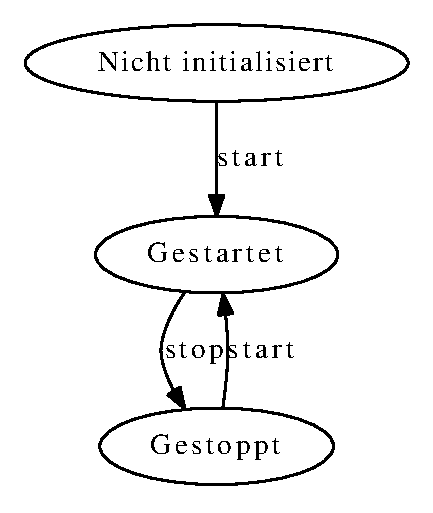
\includegraphics[width=0.15\textwidth]{graphics/tcp_stm.dot.eps}
  \caption{Verhalten einer Filetransfer-Verbindung}
  \label{filetransfer_behaviour}
\end{center}
\end{figure}

\subsubsection{SimpleWebshop-Verhalten}

%\usepackage{graphics} is needed for \includegraphics
\begin{figure}[htp]
\begin{center}
  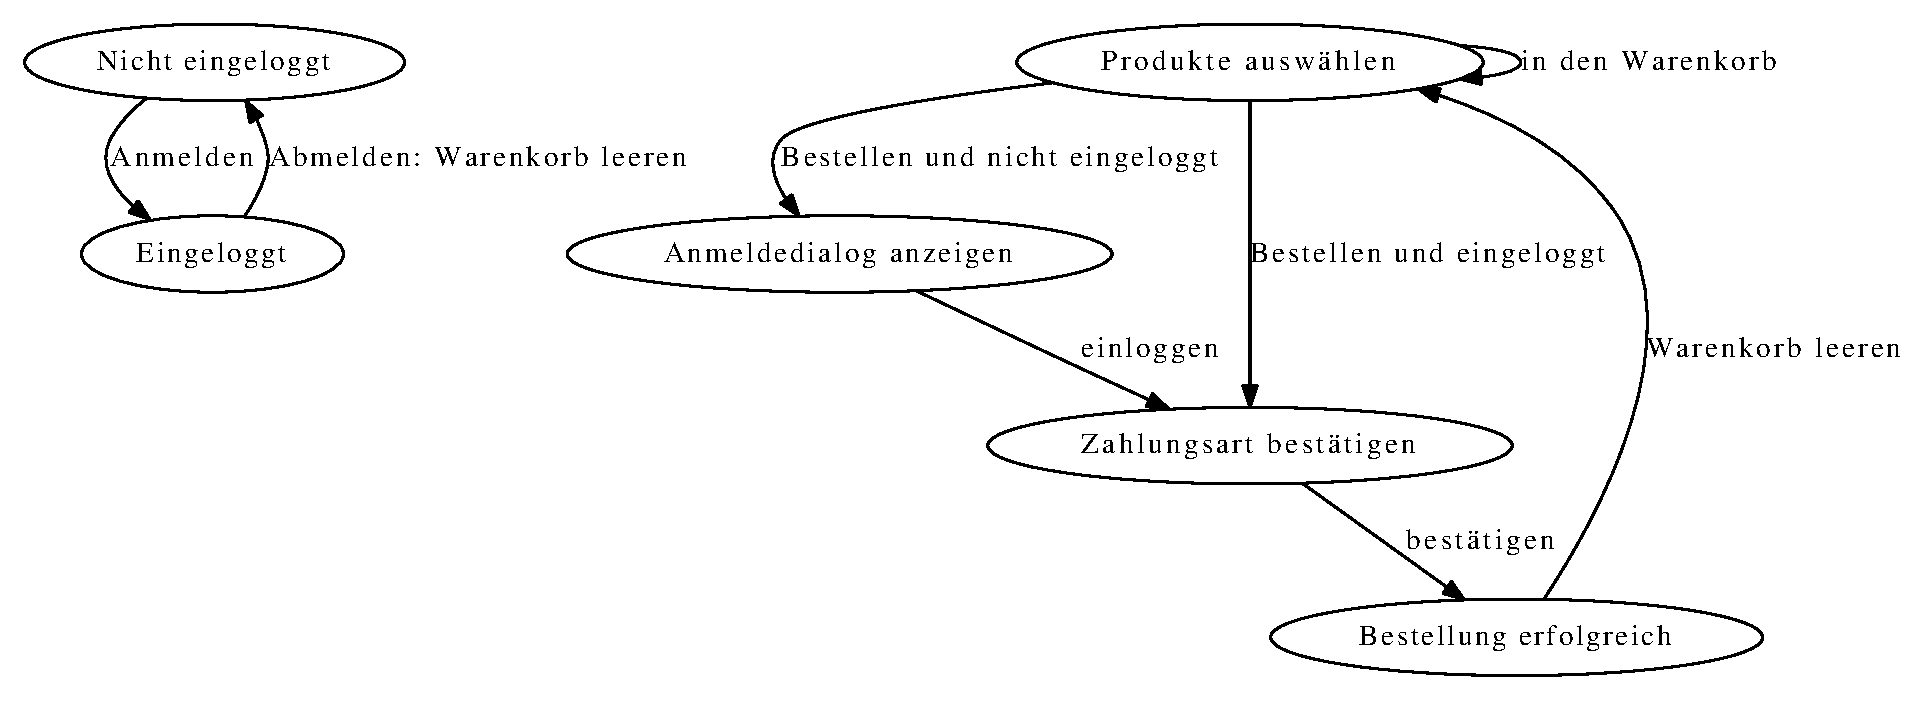
\includegraphics[width=0.6\textwidth]{graphics/webshop.dot.eps}
  \caption{Bestellvorgang in einem Web-Shop}
  \label{webshop_behaviour}
\end{center}
\end{figure}

\section{Resümee}
Durch die Verwendung von Intervall-Events kann man zustandsbasierte
Probleme deklarativ lösen. Man spart sich dann die imperative Implementierung
eines Zustandsautomaten. Dies verbessert die Verständlichkeit des Quellcodes und
verringert somit die Wartungskosten für ein Software-Projekt. 

Allerdings bringt die Verwendung von Intervall-Events auch Probleme mit sich.
Die Deregistrierung von Events obliegt nämlich dem Benutzer. Wenn ein Benutzer
nicht länger benötigte Events nicht wieder vom Event-Graph abkoppelt, dann
können die zu den Events gehörenden Objekte nicht freigegeben werden. Dies hat
zur Folge, dass der Speicherverbrauch der Anwendung möglicherweise immer weiter
ansteigt. 

Die Intervall-Events können nicht automatisch deregistriert werden, da nicht
bekannt ist, ob der Benutzer noch Interesse am Intervall-Event hat. Es könnte
sein, dass ein Intervall-Event nur ein einziges mal für den Benutzer von
Interesse ist. Möglicherweise benötigt der Benutzer das Intervall-Event aber
mehrfach. Wichtig ist daher, dem Benutzer die Deregistrierung der Events
nahezulegen.

\section{Ausblick}
Der nachfolgende Ausblick betrifft Events im Allgemeinen und Intervall-Events im
speziellen.

Zukünftig sollte sich die Intervall-Events-Library in zwei Richtungen
weiterentwickeln. Zum einen ist es wichtig den Benutzer bei der Deregistrierung
von nicht mehr benötigten Intervall-Events zu unterstützen. Und zum anderen kann
die Intervall-Events-Library ihr volles Potential nur ausspielen, wenn
die Implementierung effizient in Multithreading-Szenarien funktioniert.

\subsection{Konzepte zur Vereinfachung der Deregistrierung von Reactions}

Möglicherweise könnte man eine Datenfluss-Analyse im Kontrollfluss-Graph
vornehmen, um nach Events zu suchen. Wenn ein Event gefunden wurde, auf den eine Reaction
registriert wurden, muss sichergestellt werden, dass auch eine Reaction wieder
entfernt wird. Allerdings ist das ein "`Best-Efford"'-Ansatz. Man kann auf diese
Weise nicht in allen Fällen sicherstellen, dass die verwendeten Events immer
korrekt aufgeräumt werden.

Außerdem könnte man dem Benutzer Zugriff auf den Funktionszeiger von
anonymen Funktionen bereitstllen. Wenn Intervall-Events in Methoden verwendet
werden, sind diese Intevalle dann meist nur selten aktiv und müssen nach 
zeitlich kurzer Zeit wieder deregistriert werden. Allerdings sollten dabei 
keine anonymen Funktionen verwendet werden. Anonyme Funktionen können nämlich 
nicht deregistriert werden, da keine Möglichkeit besteht, an den Funktionszeiger
der anonymen Funktion zu kommen, um diese wieder zu deregistrieren.

\subsection{Effiziente und skalierbare Funktionsweise in
Multithreading-Szenarien}
Die Threadsicherheit ist eine überaus wünschenswerte Eigenschaft für
Intervall-Events. In der Zukunft werden Interaktionen zwischen verschiedenen 
Thread zunehmend immer wichtiger. Das Konzept der Events und der
Intervall-Events ist natürlich nicht auf sequenzielle Prozesse beschränkt und
skaliert sehr gut auch auf Thread- und Prozess-Ebene. Diese Tatsache
manifestiert sich in der Existenz von Messageoriented
Middleware. 

Um die Intervall-Events-Implementierung Multithreading-sicher zu machen, muss
geprüft werden, ob alle Zustandsänderungen des Aktiv-Zustands eines
Intervall-Events multithreading-sicher sind. Weiterhin muss die Events-Library
Multithreading-sicher sein.

\listoffigures\addcontentsline{toc}{section}{\listfigurename}
\end{document}
